\documentclass{beamer}

\usepackage[utf8]{inputenc}
\usepackage{fancybox,fancyvrb}
\usepackage{environ}
\usepackage{tikz}

\beamertemplatenavigationsymbolsempty
\setbeamertemplate{footline}[frame number]

\title{2.1 Solution Curves (Without a Solution)}

\subtitle{a lesson for MATH F302 Differential Equations}

\author{Ed Bueler, Dept.~of Mathematics and Statistics, UAF}

\date{\tiny \today}


\usetheme{Pittsburgh}


\begin{document}

\setbeamertemplate{itemize item}{$\bullet$}
\setbeamertemplate{itemize subitem}{$\circ$}


\begin{frame}
\titlepage

\centerline{\tiny for textbook: \, D. Zill, \emph{A First Course in Differential Equations with Modeling Applications}, 11th ed.}
%\color{green!40!blue}
\end{frame}


\begin{frame}{meaning of a differential equation}

\begin{itemize}
\item start over on the meaning of a (first-order) DE:
    $$\frac{dy}{dx} = f(x,y)$$

\vspace{-2mm}
    \begin{enumerate}
    \item the left side is the \emph{slope} of the solution $y(x)$
    \item given a point $(x,y)$, the right side computes a number $f(x,y)$
    \end{enumerate}
\item thus a differential equation (DE) says:
    $$\begin{matrix}
    \text{the slope of the} \\
    \text{solution } y(x) 
    \end{matrix} \quad \stackrel{\text{equals}}{=} \quad
    \begin{matrix}
    \text{a known function of} \\
    \text{the location } (x,y)
    \end{matrix}$$
\item this literal reading of the DE means that

\centerline{\alert{we can \emph{draw} a picture of the DE itself}}

\item \dots whether or not we can do the calculus/algebra to find a formula for $y(x)$
\end{itemize}
\end{frame}


\begin{frame}{direction field}

\begin{itemize}
\item \emph{main idea}: DE $\frac{dy}{dx} = f(x,y)$ should be read as computing a slope $m=\frac{dy}{dx}$ at each  point $(x,y)$
\item \dots so we create a \emph{direction field} or \emph{slope field}:
    \begin{enumerate}
    \item generate a grid of point in the $x$,$y$ plane
    \item for each point, draw a short line with the slope given by $f(x,y)$ at that point
    \end{enumerate}
\item see also: \small \href{https://en.wikipedia.org/wiki/Slope_field}{\color{cyan} \texttt{en.wikipedia.org/wiki/Slope\_field}} \normalsize

\bigskip
\item \begin{minipage}[t]{0.375\textwidth}
\emph{Example.}  By hand, draw a direction field for
$$\frac{dy}{dx} = x-y$$
on the square
$$-3 \le x \le 3, -3 \le y \le 3$$
\end{minipage} 

\vspace{20mm}
\end{itemize}
\end{frame}


\begin{frame}{computers are useful}

\begin{itemize}
\item I acknowledge \emph{happily} that this is a job for a computer
    \begin{itemize}
    \item for computer tools,  see ``found online'' at the \href{https://bueler.github.io/math302/week2.html}{\color{cyan} Week 2 tab}
    \end{itemize}

\medskip
\item \emph{Example.}  Use a computer to draw a direction field for
$\frac{dy}{dx} = x-y$ on the square $-3 \le x \le 3, -3 \le y \le 3$

\bigskip
\emph{Solution}:

\vspace{-3mm}
\hfill 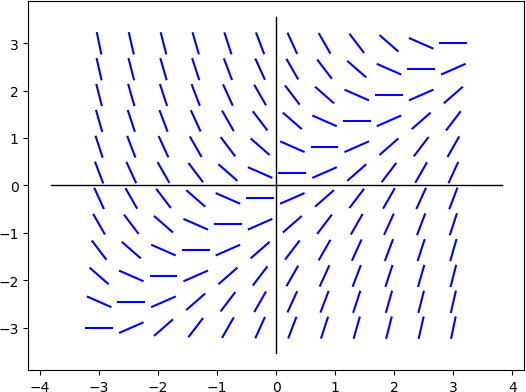
\includegraphics[width=0.5\textwidth]{figs/example-field} \phantom{as dfjadl dsf}

\medskip
\scriptsize
\texttt{def f(x,y):  return x - y}  \hfill $\longleftarrow$ \emph{from my Python code}

\texttt{dirfield(f,[-3,3,-3,3],mx=12,my=12)}
\end{itemize}
\end{frame}


\begin{frame}{picturing ODE IVPs}

\begin{itemize}
\item recall that we are often solving initial value problems
\item \emph{next main idea}:  one can \emph{see} the solution to an ODE IVP by plotting the initial point in the plane and then following the direction field from that point

\bigskip
\item \begin{minipage}[t]{0.32\textwidth} \small
\emph{Example.}  Use the direction field for
$\frac{dy}{dx} = x-y$ to sketch the solution of
    $$\frac{dy}{dx} = x-y, \, y(0)=2$$
\end{minipage}

\vspace{-25mm}
\hfill 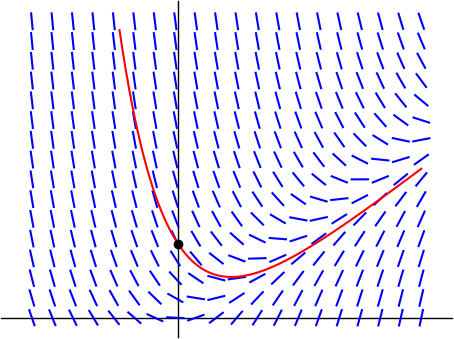
\includegraphics[width=0.55\textwidth]{figs/example-field-solution}
\end{itemize}
\end{frame}


\begin{frame}{exercise 9 in \S 2.1}

\begin{columns}
\begin{column}{0.45\textwidth}
\small
\noindent \textbf{9}.  \emph{Use computer software to obtain a direction field for the given differential equation.  By hand, sketch an approximate solution curve passing through each of the given points.}

$$\frac{dy}{dx} = 0.2 x^2 + y$$

\noindent \textbf{(a)} \quad $y(0)=\tfrac{1}{2}$

\noindent \textbf{(b)} \quad $y(2)=-1$

\vspace{10mm}

\tiny
\texttt{def f(x,y):}

\hspace{3mm} \texttt{return 0.2*x**2 + y}

\texttt{dirfield(f,[-2,5,-3,3],mx=12,my=12)}
\end{column}
\begin{column}{0.55\textwidth}

\hspace{-10mm} 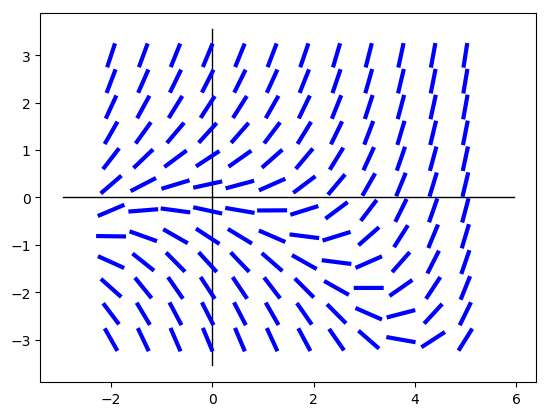
\includegraphics[width=1.15\textwidth]{figs/exercise-9-2-1}
\end{column}
\end{columns}
\end{frame}


\begin{frame}{two topics in \S 2.1}

\begin{itemize}
\item there are two topics in \S 2.1:
    \begin{itemize}
    \item direction fields for 1st-order DEs
    \item autonomous 1st-order DEs
    \end{itemize}
\item \emph{in practice: equally-important topics!}
\item both topics are about \emph{picturing DEs}, but ``autonomous'' is a special case where we can draw two kinds of pictures
\end{itemize}
\end{frame}


\begin{frame}{autonomous first-order DEs}

\begin{itemize}
\item \emph{definition}. a first-order differential equation is \emph{autonomous} if the function does not depend on the independent variable:
    $$\frac{dy}{dx} = f(y)$$

\vspace{-2mm}
    \begin{itemize}
    \item ``autonomous'' means ``independent of direct control''
    \item autonomous DE is not directly controlled by input variable $x$
    \item \dots but the \emph{solution} $y(x)$ is still a function of $x$
    \end{itemize}
\item Example.
    $$\frac{dy}{dx} = \sqrt{\sin(y)}$$
\item Non-example.
    $$\frac{dy}{dx} = x-y$$
\end{itemize}
\end{frame}


\begin{frame}{classification of first-order DEs}

\begin{itemize}
\item we will see that ``autonomous'' means ''easy to visualize''
\item using definitions from sections 1.1 and 2.1 we already have a \emph{classification} of first-order DEs:

\medskip
\begin{center}
\begin{tabular}{c|c|c}
 & autonomous & nonautonomous \\ \hline
linear \Large\strut & $y' = c\, y + d$ & $y' + P(x) y = g(x)$ \\ \hline
nonlinear \Large\strut & $y' = f(y)$ & $y'=f(x,y)$
\end{tabular}
\end{center}

\medskip
    \begin{itemize}
    \item which can we already solve by guess-and-check?
    \end{itemize}
\end{itemize}

\vspace{20mm}
\end{frame}


\begin{frame}{picturing autonomous DEs}

\begin{itemize}
\item the direction field of an autonomous DE is redundant
\item it can be simplified into a one-dimensional \emph{phase portrait} or \emph{phase line}

\medskip
\item \begin{minipage}[t]{0.36\textwidth} \small
Example.  Use a computer to draw the direction field for $x \in [-3,3]$ and $y\in [-\pi,\pi]$.  Then simplify the direction field into a phase portrait. 
    $$\frac{dy}{dx} = \cos(2y)$$
\end{minipage}

\vspace{-36mm}
\hfill 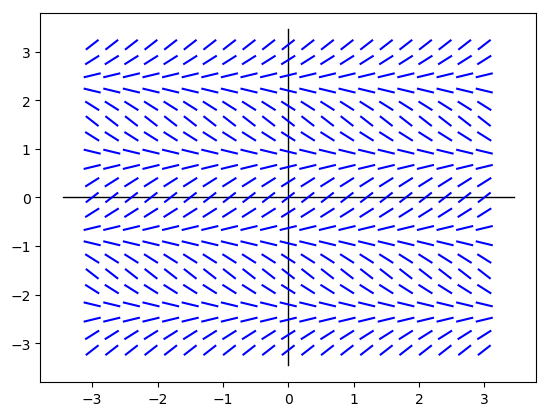
\includegraphics[width=0.45\textwidth]{figs/autonomous-cos} \phantom{dfjsdf}
% import numpy as np
% def f(x,y):  return np.cos(2*y)
% df.dirfield(f,[-3,3,-np.pi,np.pi],mx=21,my=21,slopeslinewidth=1.5)
\end{itemize}
\end{frame}


\begin{frame}{critical points of autonomous DEs}

\begin{itemize}
\item a value $y=c$ of an autonomous first-order DE
    $$\frac{dy}{dx} \stackrel{(\ast)}{=} f(y)$$
is called a \emph{critical point} if $f(c)=0$
    \begin{itemize}
    \item a.k.a.~\emph{equilibrium point} or \emph{stationary point}
    \end{itemize}

\medskip
\item if $y=c$ is a critical point of ($\ast$) then $y=c$ is a solution of ($\ast$)

\medskip
\item Example.  $y=\pi/4$ is a critical point \emph{and a solution} of
    $$\frac{dy}{dx} = \cos(2y)$$

\vspace{5mm}
\end{itemize}
\end{frame}


\begin{frame}{example}

\begin{itemize}
\small
\item \begin{minipage}[t]{0.4\textwidth}
Example.  By hand, sketch the phase portrait of
   $$\frac{dz}{dt} = z + z^3$$
and show all critical points.  Then sketch the graph of solutions to the ODE IVP with the following initial values.
    \begin{itemize}
    \item[\color{black} \textbf{(a)}] $z(0)=1$
    \item[\color{black} \textbf{(b)}] $z(0)=-1/2$
    \item[\color{black} \textbf{(c)}] $z(0)=-1$
    \item[\color{black} \textbf{(c)}] $z(0)=-2$
    \end{itemize}
\end{minipage}
\end{itemize}
\end{frame}


\begin{frame}{classifying critical points}

\begin{itemize}
\item X
\end{itemize}
\end{frame}


\begin{frame}{exercise 27 in \S 2.1}

\begin{itemize}
\item X
\end{itemize}
\end{frame}


\begin{frame}{exercise 40 in \S 2.1}

\begin{itemize}
\item X
\end{itemize}
\end{frame}


\begin{frame}{X}

\begin{itemize}
\item X
\end{itemize}
\end{frame}


\begin{frame}{looking ahead: next two sections 2.2, 2.3}

\begin{itemize}
\item X
\end{itemize}

\begin{tabular}{c|c|c}
 & autonomous & nonautonomous \\ \hline
linear \Large\strut & $y' = c\, y + d$ & $y' + P(x) y = g(x)$ \\ \hline
nonlinear \Large\strut & $y' = f(y)$ & 

\begin{minipage}{45mm}
\medskip

\small
    \begin{tabular}{c|c}
    separable & nonseparable \\ \hline
    $y'=g(x)h(y)$ & $y'=f(x,y)$
    \end{tabular}
\end{minipage}
\end{tabular}
\end{frame}


\begin{frame}{expectations}

to learn this material, just watching this video is \emph{not} enough; also
\begin{itemize}
\item see ``found online'' videos and direction-field plotters at

\centerline{\href{https://bueler.github.io/math302/week2.html}{\tt \color{cyan} bueler.github.io/math302/week2.html}}
\item \emph{read} section 2.1 in the textbook
    \begin{itemize}
    \item a large new vocabulary in this section
    \item the language of \emph{qualitative} differential equations
    \item I did not cover ``translation property'' on page 43; read that!
    \end{itemize}
\item \emph{do} the WebAssign exercises for section 2.1
    \begin{itemize}
    \item get more out of these by \emph{not} using the internet to cheat!
    \end{itemize}
\item you \emph{don't} have to know programming to do this class
    \begin{itemize}
    \item \dots but interacting with the computer is obligatory!
    \item find tools (e.g.~\href{https://www.desmos.com/}{\color{cyan} desmos} or \href{https://www.wolframalpha.com/}{\color{cyan} Wolfram alpha}) to do jobs
    \item I will show a few lines of Matlab or Python when there is a  computer-suitable job
    \end{itemize}
\end{itemize}
\end{frame}

\end{document}

